% !TeX root = RJwrapper.tex
\title{Article Proposal: Concise indicator variable recoding with ind2cat}
\author{by Evangeline Reynolds}

\maketitle

\abstract{%
Indicator variables are easy to create, store, and interpret
\citep{10.1177/1536867X19830921}. They concisely encode information
about the presence or not of a condition for observational units. The
variable name encapsulates the information about the condition of
interest, and the variable's values (TRUE and FALSE, 1 or 0, ``Yes'' or
``No'') indicate if the condition is met for the observational unit.
When using indicator variables to use in summary products, analysts
often make a choice between using an indicator variable as-is or
crafting categorical variables where values can be directly interpreted.
Using the indicator variable as-is may be motivated by time savings, but
yields poor results in summary products. \{\{ind2cat\}\} can help
analysts concisely translate indicator variables to categorical
variables for reporting products, yielding more polished outputs. By
default, ind2cat creates the categorical variable from the indicator
variable name, resulting in a light weight syntax.
}

\hypertarget{introduction}{%
\section{Introduction}\label{introduction}}

Using current analytic tools analysts make a choice between directly
using indicators or verbose recode. Current procedures for recoding
indicator variables to a categorical variable is repetitive, but
forgoing a recode and using indicator variables directly yields
hard-to-interpret summary products.

Below is demonstrated how an analyst might current recode and indicator
variable; this method is repetitive:

\begin{Schunk}
\begin{Sinput}
library(tidyverse)
tidytitanic::passengers %>% 
  tibble() %>% 
  mutate(cat_survived = ifelse(survived, 
                               "survived", 
                               "not survived"), 
         .before = 1)
\end{Sinput}
\begin{Soutput}
     # A tibble: 1,313 x 6
        cat_survived name                                   class   age sex   survi~1
        <chr>        <chr>                                  <chr> <dbl> <chr>   <int>
      1 survived     Allen, Miss Elisabeth Walton           1st   29    fema~       1
      2 not survived Allison, Miss Helen Loraine            1st    2    fema~       0
      3 not survived Allison, Mr Hudson Joshua Creighton    1st   30    male        0
      4 not survived Allison, Mrs Hudson JC (Bessie Waldo ~ 1st   25    fema~       0
      5 survived     Allison, Master Hudson Trevor          1st    0.92 male        1
      6 survived     Anderson, Mr Harry                     1st   47    male        1
      7 survived     Andrews, Miss Kornelia Theodosia       1st   63    fema~       1
      8 not survived Andrews, Mr Thomas, jr                 1st   39    male        0
      9 survived     Appleton, Mrs Edward Dale (Charlotte ~ 1st   58    fema~       1
     10 not survived Artagaveytia, Mr Ramon                 1st   71    male        0
     # ... with 1,303 more rows, and abbreviated variable name 1: survived
\end{Soutput}
\end{Schunk}

\begin{Schunk}
\begin{Sinput}
tidytitanic::passengers %>% 
ggplot() + 
  aes(x = sex) + 
  geom_bar() + 
  facet_grid(~ ifelse(survived, 
                      "survived", 
                      "not survived")) 
\end{Sinput}

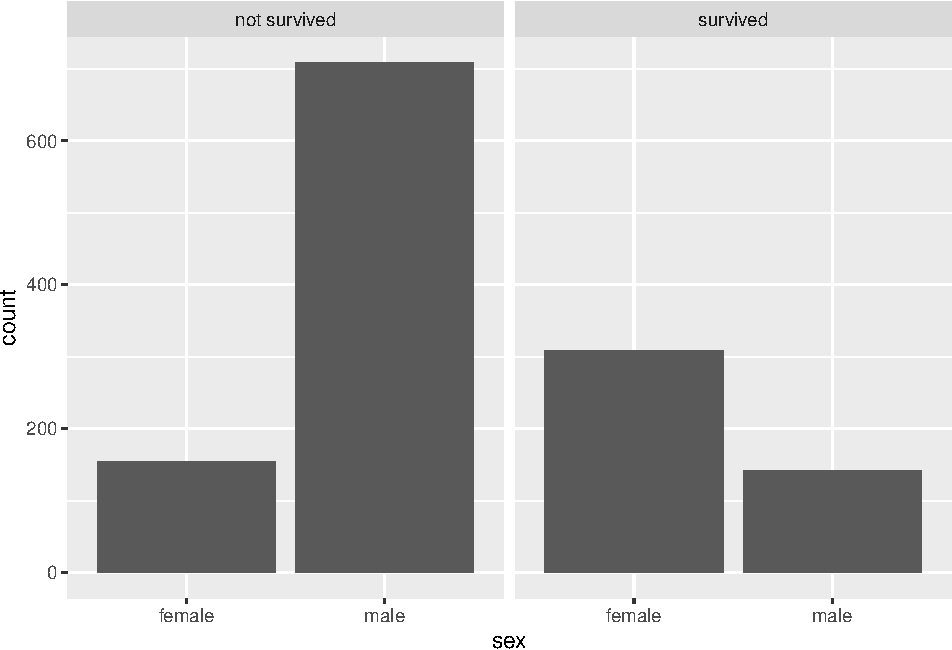
\includegraphics[width=0.69\linewidth]{r_journal_files/figure-latex/visual_status_quo-1} \end{Schunk}

This solution above also does not address category display ordering;
ordering in products will be alphabetical and not reflect the F/T order
of the source variable. An additional step to reflect the source
variable, using a function like forcats::fct\_rev, may be required for
consistency in reporting.

\begin{Schunk}
\begin{Sinput}
data.frame(ind_daytime = c(T, F, T, T)) %>% 
    mutate(cat_survived = ifelse(ind_daytime, "daytime", "not daytime")) %>% 
  mutate(cat_survived = fct_rev(cat_survived)) %>% 
  ggplot() + 
  aes(x = cat_survived) + 
  geom_bar()
\end{Sinput}

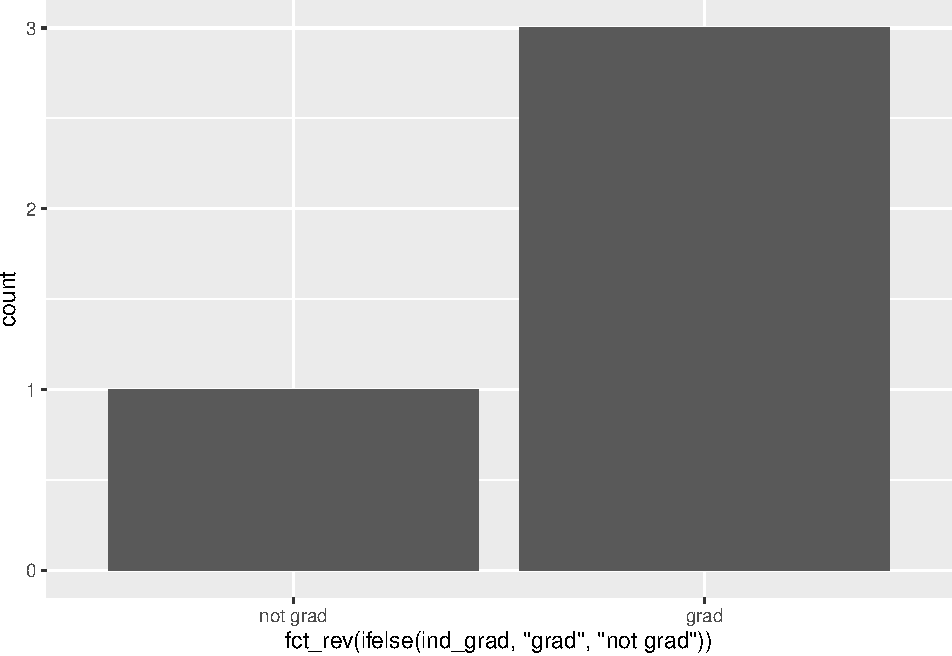
\includegraphics[width=0.69\linewidth]{r_journal_files/figure-latex/visual_status_quo_order-1} \end{Schunk}

Given how verbose recoding can be, analyst may choose to forego a
recoding the variable, especially in exploratory analysis.

However, when indicator variables are used directly in data summary
products like tables and visuals, information is often awkwardly
displayed and is sometimes lost.

Below, the column header comes from the indicator variable name allowing
savvy readers to interpret the output, but interpretation is awkward:

\begin{Schunk}
\begin{Sinput}
tidytitanic::passengers %>% 
  count(survived) 
\end{Sinput}
\begin{Soutput}
       survived   n
     1        0 863
     2        1 450
\end{Soutput}
\end{Schunk}

In the following two-way table, information is completely lost due to
using the indicator variable directly:

\begin{Schunk}
\begin{Sinput}
tidytitanic::passengers %>% 
  janitor::tabyl(sex, survived)
\end{Sinput}
\begin{Soutput}
         sex   0   1
      female 154 308
        male 709 142
\end{Soutput}
\end{Schunk}

In the following visual summary of the data, where the indicator
variable is directly used, interpretation is awkward.

\begin{Schunk}
\begin{Sinput}
library(tidyverse)

tidytitanic::passengers %>% 
  ggplot() + 
  aes(x = survived) + 
  geom_bar()
\end{Sinput}
\begin{figure}
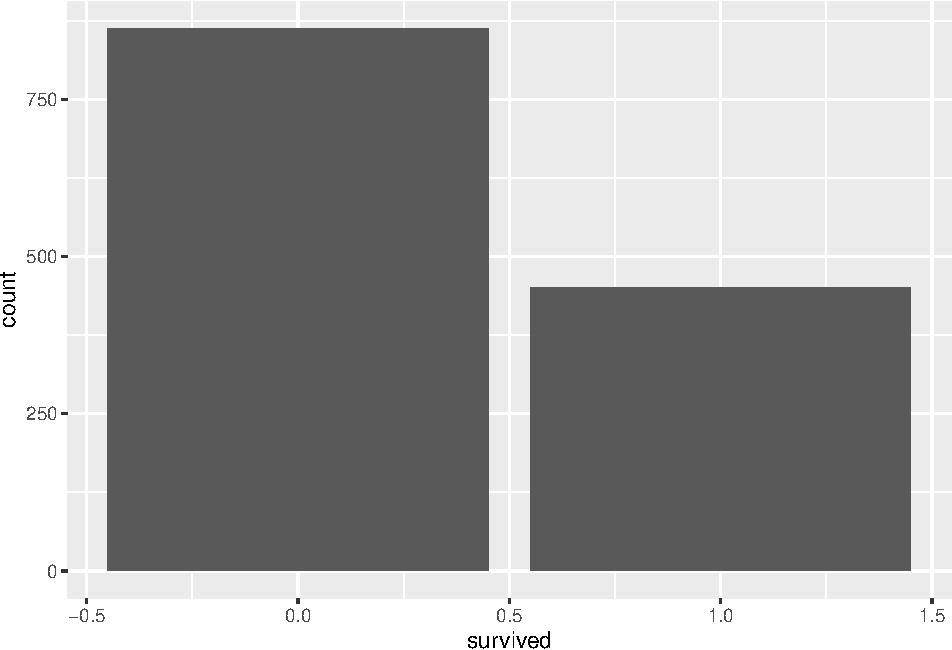
\includegraphics[width=0.69\linewidth]{r_journal_files/figure-latex/direct_visual_awkward-1} \caption[A]{A. Bar labels + axis label preserves information but is awkward}\label{fig:direct_visual_awkward}
\end{figure}
\end{Schunk}

If used as a faceting variable with the ggplot2 library, information is
lost and the graph is not directly interpretable.

\begin{Schunk}
\begin{Sinput}
tidytitanic::passengers %>% 
ggplot() + 
  aes(x = age) + 
  geom_histogram() + 
  facet_grid(~ survived)
\end{Sinput}
\begin{figure}
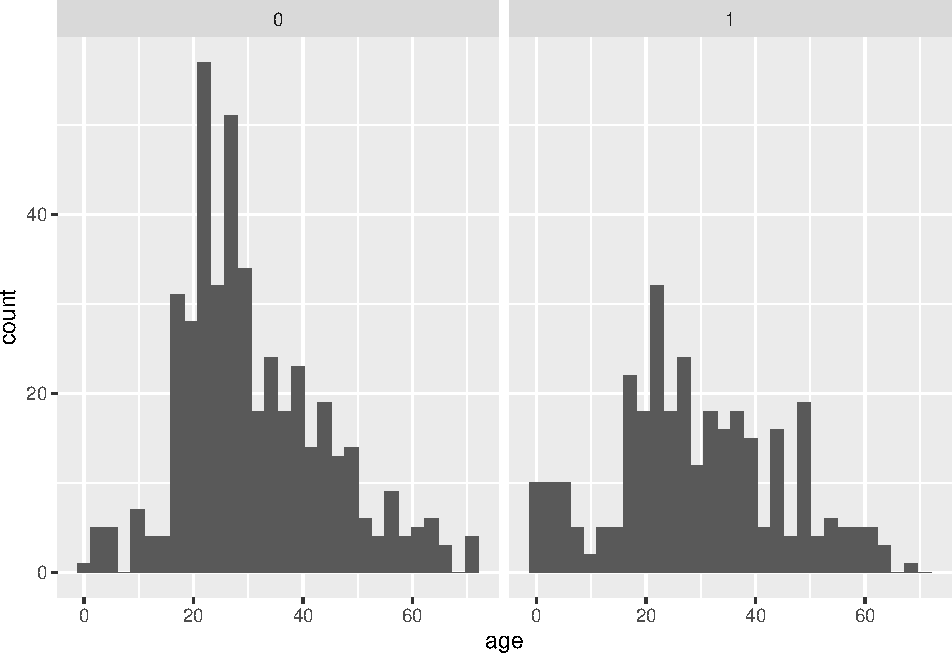
\includegraphics[width=0.69\linewidth]{r_journal_files/figure-latex/direct_visual_loss-1} \caption[D]{D. Facetting directly on an indicator variable with popular ggplot2 results in information loss}\label{fig:direct_visual_loss}
\end{figure}
\end{Schunk}

\hypertarget{introducing-ind2catind_recode}{%
\section{Introducing
ind2cat::ind\_recode}\label{introducing-ind2catind_recode}}

The ind2cat::ind\_recode() function uses variable name to automatically
derive human-readable, and appropriately ordered categories.

To clearly compare the new method, we reiterate the status quo with a
toy example:

\begin{Schunk}
\begin{Sinput}
library(tidyverse)

data.frame(ind_graduated = 
             c(TRUE, TRUE, FALSE))  %>% 
  mutate(cat_graduated  = 
           ifelse(ind_graduated, 
                  "graduated", 
                  "not graduated"))  %>% 
  mutate(cat_graduated = 
           fct_rev(cat_graduated)
         )  
\end{Sinput}
\begin{Soutput}
       ind_graduated cat_graduated
     1          TRUE     graduated
     2          TRUE     graduated
     3         FALSE not graduated
\end{Soutput}
\end{Schunk}

Below we contrast this with the use of ind2cat's ind\_recode function
which avoids repetition by creating categories based on the indicator
variable name. Using the the function ind\_recode(), we can accomplish
the same task shown above more succinctly:

\begin{Schunk}
\begin{Sinput}
library(ind2cat)

data.frame(ind_graduated = 
             c(TRUE, TRUE, FALSE)) %>% 
  mutate(cat_graduated  = 
           ind_recode(ind_graduated)
         )
\end{Sinput}
\begin{Soutput}
       ind_graduated cat_graduated
     1          TRUE     graduated
     2          TRUE     graduated
     3         FALSE not graduated
\end{Soutput}
\end{Schunk}

The indicator variable can be populated with TRUE/FALSE values as well
as 1/0 or ``Yes''/``No'' (and variants `y/n' for example).

Furthermore, while ind\_recode default functionality allows analysts to
move from its first-cut human-readable recode, it also allows fully
customized categories via adjustment of the functions parameters.

\begin{itemize}
\item
  cat\_true a character string string to be used place of T/1/``Yes''
  for the categorical variable output, if NULL the category is
  automatically generated from the variable name
\item
  negator a character string used to create cat\_false when cat\_false
  is NULL, default is `not'
\item
  cat\_false a character string string to be used place of F/0/``No''
  for the categorical variable output, if NULL the category is
  automatically generated from cat\_true and the negator
\item
  rev logical indicating if the order should be reversed from the F/T
  ordering of the indicator source variable, default is FALSE
\item
  var\_prefix a character string that will be ignored when creating the
  categorical variable
\end{itemize}

\begin{Schunk}
\begin{Sinput}
data.frame(ind_graduated = c(T,T,F)) %>% 
  mutate(cat_graduated  = ind_recode(ind_graduated, 
                                     cat_false = "current"))
\end{Sinput}
\begin{Soutput}
       ind_graduated cat_graduated
     1          TRUE     graduated
     2          TRUE     graduated
     3         FALSE       current
\end{Soutput}
\end{Schunk}

\begin{Schunk}
\begin{Sinput}
tibble(ind_grad = c("y", "n")) %>%
  mutate(cat_grad  = ind_recode(ind_grad, 
                                cat_true = "graduated"))
\end{Sinput}
\begin{Soutput}
     # A tibble: 2 x 2
       ind_grad cat_grad     
       <chr>    <fct>        
     1 y        graduated    
     2 n        not graduated
\end{Soutput}
\end{Schunk}

\begin{Schunk}
\begin{Sinput}
tibble(ind_grad = c(T,T,F)) %>%
  mutate(cat_grad  = ind_recode(ind_grad, negator = "didn't"))
\end{Sinput}
\begin{Soutput}
     # A tibble: 3 x 2
       ind_grad cat_grad   
       <lgl>    <fct>      
     1 TRUE     grad       
     2 TRUE     grad       
     3 FALSE    didn't grad
\end{Soutput}
\end{Schunk}

\begin{Schunk}
\begin{Sinput}
tibble(ind_grad = c("Y", "N")) %>%
  mutate(cat_grad  = ind_recode(ind_grad, cat_false = "enrolled"))
\end{Sinput}
\begin{Soutput}
     # A tibble: 2 x 2
       ind_grad cat_grad
       <chr>    <fct>   
     1 Y        grad    
     2 N        enrolled
\end{Soutput}
\end{Schunk}

\begin{Schunk}
\begin{Sinput}
tibble(ind_grad = c("yes", "no")) %>%
  mutate(cat_grad  = ind_recode(ind_grad, rev = TRUE)) %>% 
  mutate(cat_grad_num = as.numeric(cat_grad))
\end{Sinput}
\begin{Soutput}
     # A tibble: 2 x 3
       ind_grad cat_grad cat_grad_num
       <chr>    <fct>           <dbl>
     1 yes      grad                1
     2 no       not grad            2
\end{Soutput}
\end{Schunk}

\begin{Schunk}
\begin{Sinput}
tibble(dummy_grad = c(0,0,1,1,1 ,0 ,0)) %>%
  mutate(cat_grad  = ind_recode(dummy_grad, var_prefix = "dummy_"))
\end{Sinput}
\begin{Soutput}
     # A tibble: 7 x 2
       dummy_grad cat_grad
            <dbl> <fct>   
     1          0 not grad
     2          0 not grad
     3          1 grad    
     4          1 grad    
     5          1 grad    
     6          0 not grad
     7          0 not grad
\end{Soutput}
\end{Schunk}

\hypertarget{use-in-data-products-like-figures-and-tables}{%
\subsection{Use in data products like figures and
tables}\label{use-in-data-products-like-figures-and-tables}}

In what follows, we show ind2cat's use in summary products, which is a
main motivation for ind2cat.

\begin{Schunk}
\begin{Sinput}
tidytitanic::passengers %>% 
ggplot() + 
  aes(x = ind_recode(survived)) + 
  geom_bar()
\end{Sinput}

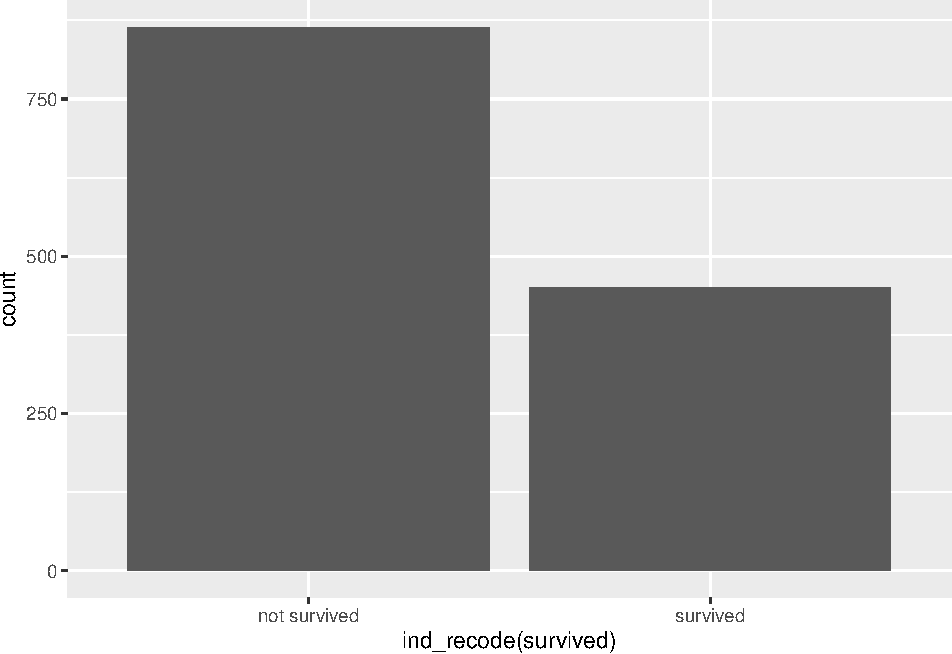
\includegraphics[width=0.69\linewidth]{r_journal_files/figure-latex/visual_ind2cat_improves-1} \end{Schunk}

\begin{Schunk}
\begin{Sinput}
# or
last_plot() +
  aes(x = ind_recode(survived, cat_false = "perished"))
\end{Sinput}

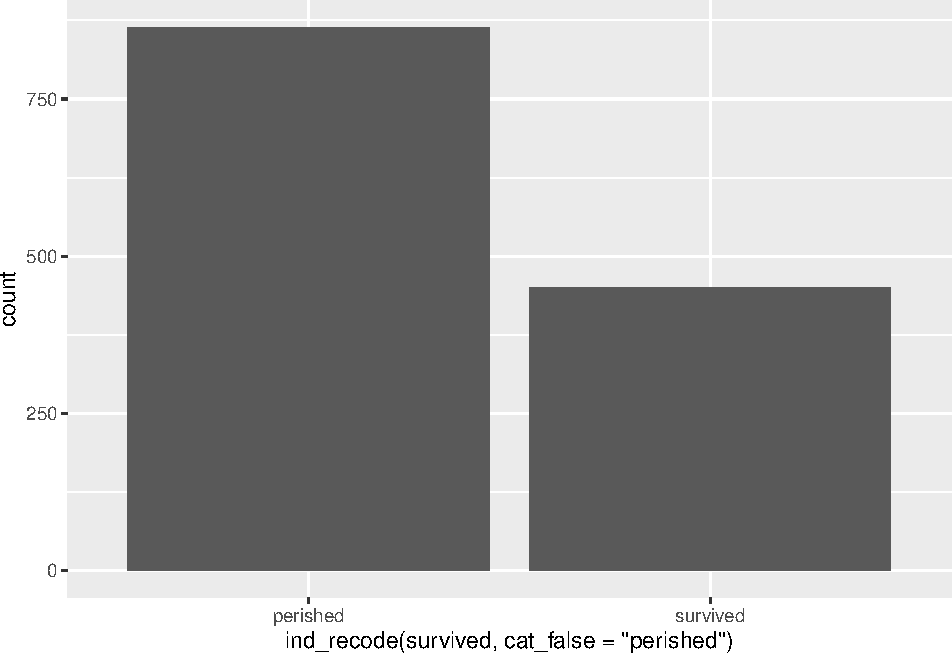
\includegraphics[width=0.69\linewidth]{r_journal_files/figure-latex/visual_ind2cat_improves_cat_false-1} \end{Schunk}

\begin{Schunk}
\begin{Sinput}
# or
last_plot() +
  aes(x = ind_recode(survived, cat_false = "didn't", rev = T)) + 
  labs(x = NULL)
\end{Sinput}

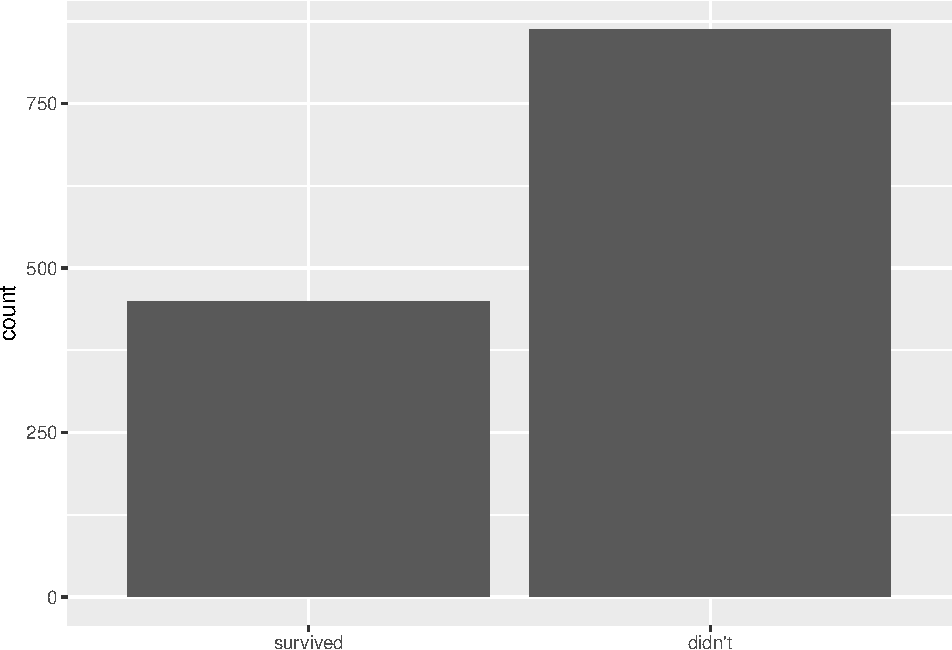
\includegraphics[width=0.69\linewidth]{r_journal_files/figure-latex/visual_ind2cat_improves_cat_false_rev-1} \end{Schunk}

\begin{Schunk}
\begin{Sinput}
tidytitanic::passengers %>% 
ggplot() + 
  aes(x = sex) + 
  geom_bar() + 
  facet_grid(~ ind_recode(survived))
\end{Sinput}

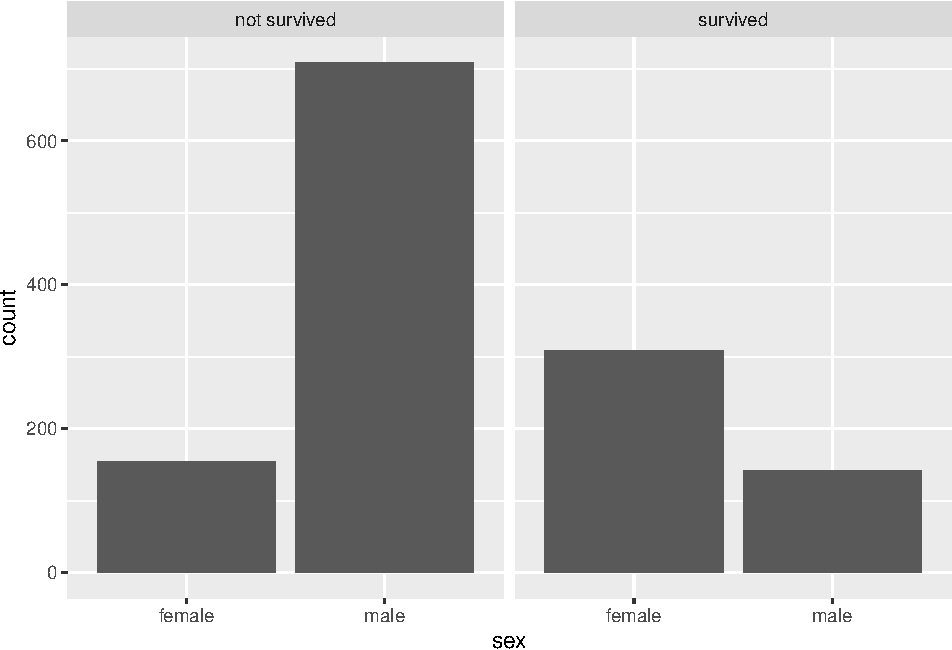
\includegraphics[width=0.69\linewidth]{r_journal_files/figure-latex/visual_ind2cat_preserves-1} \end{Schunk}

\begin{Schunk}
\begin{Sinput}
tidytitanic::passengers %>%
  mutate(cat_survived = ind_recode(survived)) %>% 
  janitor::tabyl(sex, cat_survived) %>% 
  janitor::adorn_percentages() %>% 
  janitor::adorn_pct_formatting() %>% 
  janitor::adorn_ns(position = "rear")
\end{Sinput}
\begin{Soutput}
         sex not survived    survived
      female  33.3% (154) 66.7% (308)
        male  83.3% (709) 16.7% (142)
\end{Soutput}
\end{Schunk}

\hypertarget{conclusion}{%
\section{Conclusion}\label{conclusion}}

\hypertarget{implementation-details}{%
\section{Implementation details}\label{implementation-details}}

\begin{Schunk}
\begin{Sinput}
readLines("R/ind_recode.R") -> implementation
\end{Sinput}
\end{Schunk}

\begin{Schunk}
\begin{Sinput}
#' ind_recode
#'
#' @param var the name of an indicator variable
#' @param var_prefix a character string that will be ignored when creating the categorical variable
#' @param negator a character string used to create cat_false when cat_false is NULL, default is 'not'
#' @param cat_true a character string string to be used place of  T/1/"Yes" for the categorical variable output, if NULL the category is automatically generated from the variable name
#' @param cat_false a character string string to be used place of  F/0/"No" for the categorical variable output, if NULL the category is automatically generated from the cat true and the negator
#' @param rev logical indicating if the order should be reversed from the F/T ordering of the indicator source variable, default is FALSE
#'
#' @return
#' @export
#'
#' @examples
#' library(tibble)
#' library(dplyr)
#' tibble(ind_grad = c(0,0,1,1,1 ,0 ,0)) %>%
#'   mutate(cat_grad  = ind_recode(ind_grad))
#'
#' tibble(ind_grad = c(TRUE,TRUE,FALSE)) %>%
#'   mutate(cat_grad  = ind_recode(ind_grad))
#'
#' tibble(ind_grad = c("Y", "N")) %>%
#'   mutate(cat_grad  = ind_recode(ind_grad))
#'
#' tibble(ind_grad = c("y", "n")) %>%
#'   mutate(cat_grad  = ind_recode(ind_grad))
#'
#' tibble(ind_grad = c("yes", "no")) %>%
#'   mutate(cat_grad  = ind_recode(ind_grad))
ind_recode <- function(var, var_prefix = "ind_", negator = "not",
                       cat_true = NULL, cat_false = NULL, rev = FALSE){

  if(is.null(cat_true)){
    cat_true = deparse(substitute(var)) %>%   # use r lang in rewrite
      stringr::str_remove(paste0("^", var_prefix)) %>%
      stringr::str_replace_all("_", " ")
  }

  if(is.null(cat_false)){
    cat_false = paste(negator, cat_true)
  }

  # for yes/no case
  if(is.character({{var}})){

    my_var <- {{var}} %>% as.factor() %>% as.numeric() - 1

  }else{

    my_var <- {{var}}
  }

  if(rev){
    ifelse(my_var, cat_true, cat_false) %>%
      factor(levels = c(cat_true, cat_false))
  }else{
    ifelse(my_var, cat_true, cat_false) %>%
      factor(levels = c(cat_false, cat_true))
  }


}
\end{Sinput}
\end{Schunk}

\bibliography{RJreferences.bib}

\address{%
Evangeline Reynolds\\
Affiliation\\%
line 1\\ line 2\\
%
\url{https://journal.r-project.org}\\%
\textit{ORCiD: \href{https://orcid.org/0000-0002-9079-593X}{0000-0002-9079-593X}}\\%
\href{mailto:author1@work}{\nolinkurl{author1@work}}%
}

